\section{Введение}
Центрами окраски в алмазах называют инородные атомы, внедрённые 
в кристаллическую решётку алмаза. Наиболее интересными центрами окраски
в настоящий момент являются NV-, SiV- и GeV-центры. Наличие таких центров
в кристаллической решётке приводит к люминесценции алмаза (наиболее 
выраженным свойством люминесценции обладают центры NV$^-$, SiV$^-$,
GeV$^-$, далее мы будем рассматривать именно их). Температурная
зависимость спектра излучения позволяет определять температуру алмаза,
а значит, и окружающей среды. Температурные датчики, в основе которых лежит
алмаз с центрами окраски, могут заменять обычные полупроводниковые датчики
температур, в том числе и в экстремальных условиях. Кроме того, маленький размер
таких устройств позволяет использовать их для исследования внутриклеточных 
процессов живых организмов, или, например, для исследования активности мозга.

Другим способом использования люминесценции является измерение магнитного поля.
Вследствие эффекта Зеемана наблюдается расщепление энергетических уровней 
эектронной оболочки. Зная это расщепление, можно определить величину и направление
внешнего магнитного поля. Такие датчики могут быть использованы, например, для
геологической разведки. 

\begin{figure}[!h]
    \begin{center}
        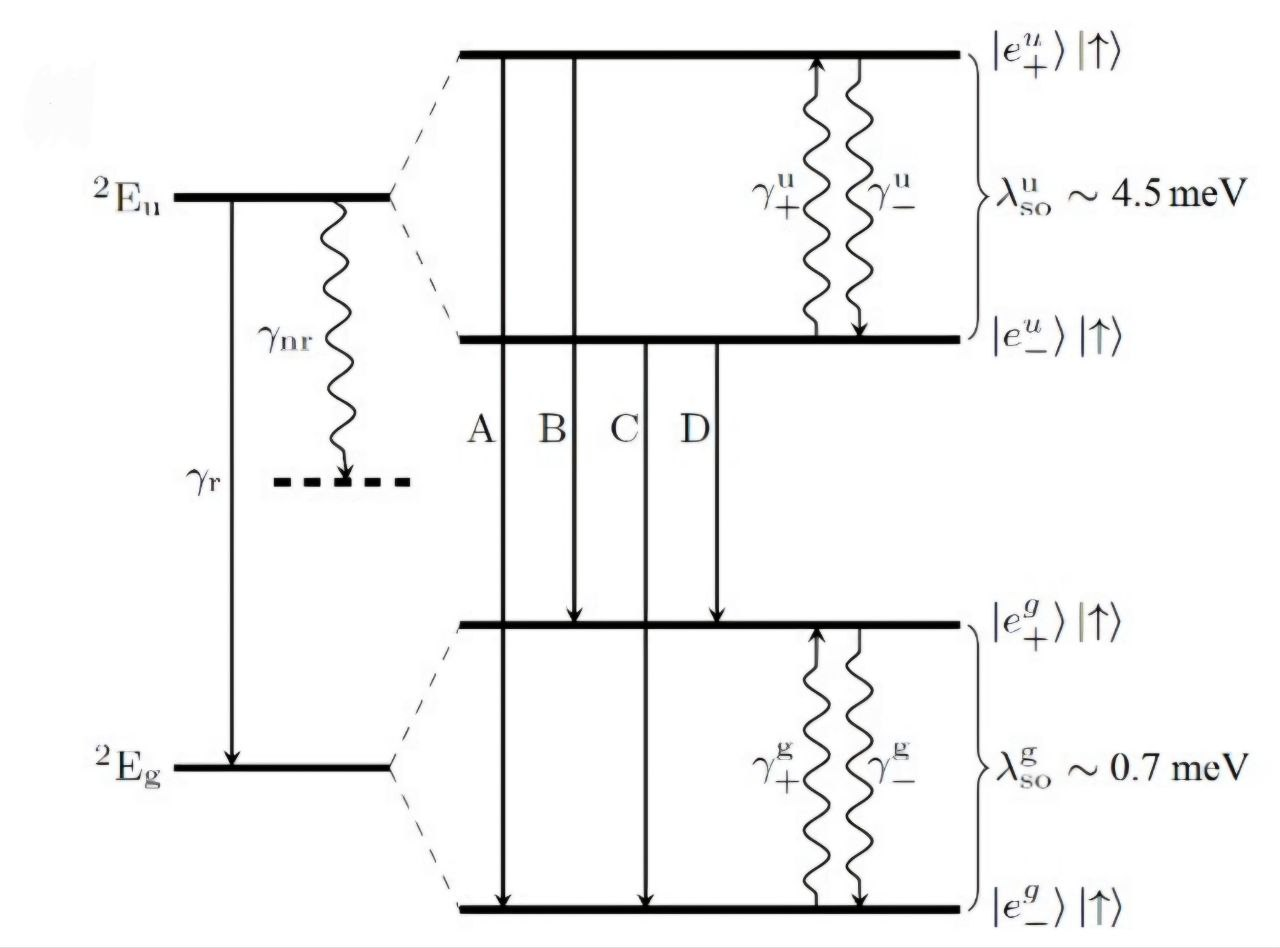
\includegraphics[width=0.7 \linewidth]{Energy levels.jpg}
        \caption{Схема уровней оптического электронного перехода в GeV-центре.
        Сплошными прямыми линией отмечены оптические переходы,
        волнистыми -- нерадиационные переходы.}
        \label{Energy levels}
    \end{center}
\end{figure}


Схема уровней оптического перехода электронной оболочки GeV-цетра представлена 
на рис. \ref{Energy levels}. Основной и первый возбуждённый уровни расщеплены на два вследствие
спин-орбитального взаимодействия: спин электронной оболочки $s_z$ = $\pm$1/2,
а момент импульса $l_z$ = $\pm$1. Каждый из этих уровней дважды вырожден.
При нулевой температуре можно наблюдать
4 линии (A, B, C и D на рис. \ref{Energy levels}), однако при повышении температуры
происходит уширение линий вследствие эффекта Яна-Теллера, и линии тонких структур
перестают быть различимыми. Этот эффект
проявляется в поглощении или испускании фонона при переходе электрона между
подуровнями тонкой структуры. На рис. \ref{J-T effect} изображены возможные переходы электрона:
в случае (a) поглощается один фонон, соответствующий энергии перехода. В случаях
(b) и (c) поглощаются 2 фонона, имеющих такие энергии, чтобы их сумма была 
равна энергии перехода. В исследуемых GeV-центрах процесс (b) не происходит.

Таким образом, приведённый эффект при известных константах позволяет определять 
температуру по ширине линии люминесценции. Кроме того, имеется зависимость 
положения пика люминесценции и расстояния между пиками от температуры. Целью
данной работы является исследование этих зависимостей для GeV-центров окраски 
алмаза.  

\begin{figure}[!h]
    \begin{center}
        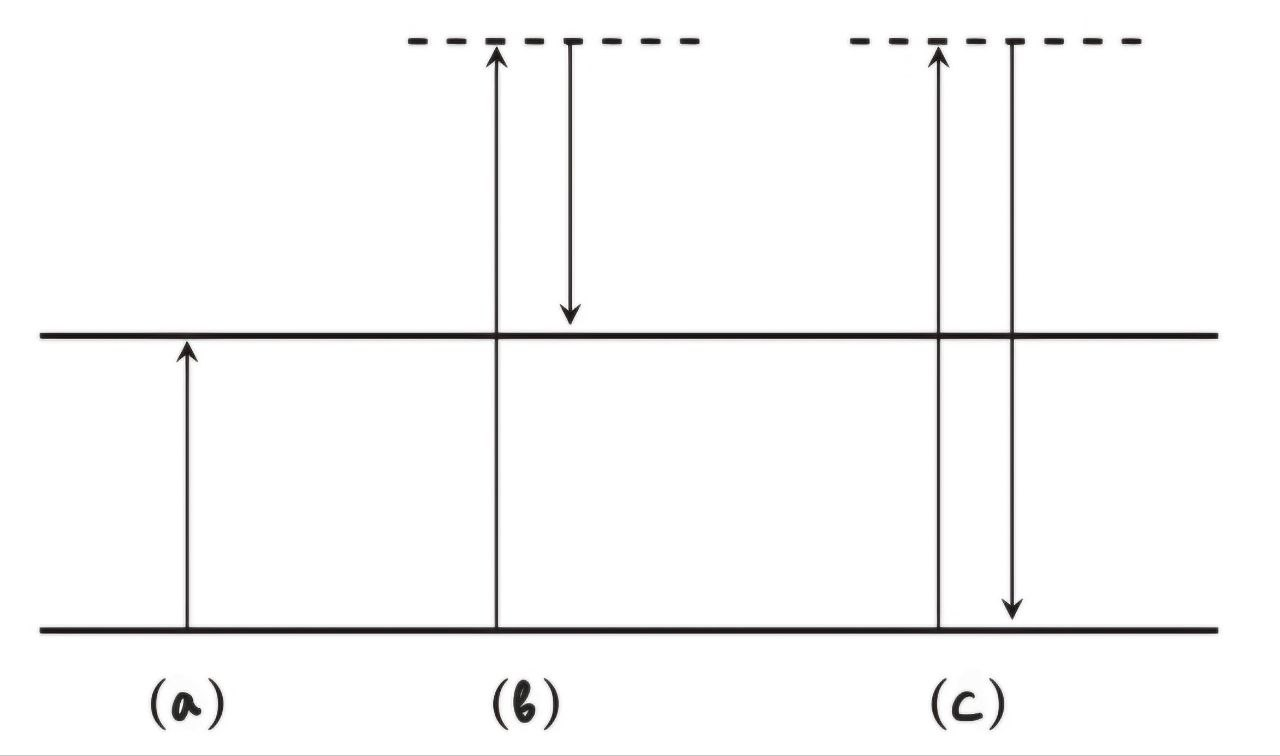
\includegraphics[width=0.5 \linewidth]{Jahn-Teller effect.jpg}
        \caption{(a) -- прямой однофононный процесс, (b) -- двухфононный
        Рамановский процесс, (c) -- упругое рассеяние фононов}
        \label{J-T effect}
    \end{center}
\end{figure}

При низких температурах ширины оптических линий шире для переходов A и B,
чем для переходов с более низкой энергией C и D. Это происходит из-за 
тепловой релаксации, сокращающей эффективное время жизни верхнего уровня
посредством скорости распада $\gamma_{-}^u$, которая быстрее, чем 
$\gamma_{+}^u$ на фактор Больцмана $\gamma_{-}^u = \gamma_{+}^u 
\exp(\lambda_{so}^u / k_B T)$.

